\begin{frame}{Future Directions of Protein Language Models}
\setbeamercovered{transparent}
    \begin{columns}
        % Left Column: Tasks
        \column{0.45\textwidth}

        \begin{center}
            \begin{tikzpicture}[
                node distance=0.3cm and 1.2cm,
                align=center,
                rounded corners,
                every node/.style={},
                input/.style={draw,  shading=axis, left color=blue!30, right color=white!30, text width=4cm, minimum height=1.5cm},
                arrow/.style={-Stealth, thick},
                scale=0.8
            ]

            % Tasks
            {\node[input, opacity=1] (structure) {Integration with Structural Data};}
            \pause
            {\node[input, below=0.5cm of structure, opacity=1] (interactions) {Advancing Zero-shot Learning};}
            \pause
            {\node[input, below=0.5cm of interactions, opacity=1] (mutation) {Efficiency Improvements};}
            \pause
            {\node[input, below=0.5cm of mutation, opacity=1]{Applications in Drug Discovery};}

        \end{tikzpicture}
        \end{center}

        % Right Column: Models
        \column{0.55\textwidth}
        \begin{center}
            \begin{tikzpicture}[
                node distance=0.3cm and 1,
                align=center,
                rounded corners,
                every node/.style={},
                input/.style={draw, fill=greyblue!40, text width=4cm, minimum height=.8cm},
                output/.style={draw,fill=white!10, text width=5cm, minimum height=.8cm},
                arrow/.style={-Stealth, thick},
                scale=0.8
            ]
            \only<1>{
                % \node {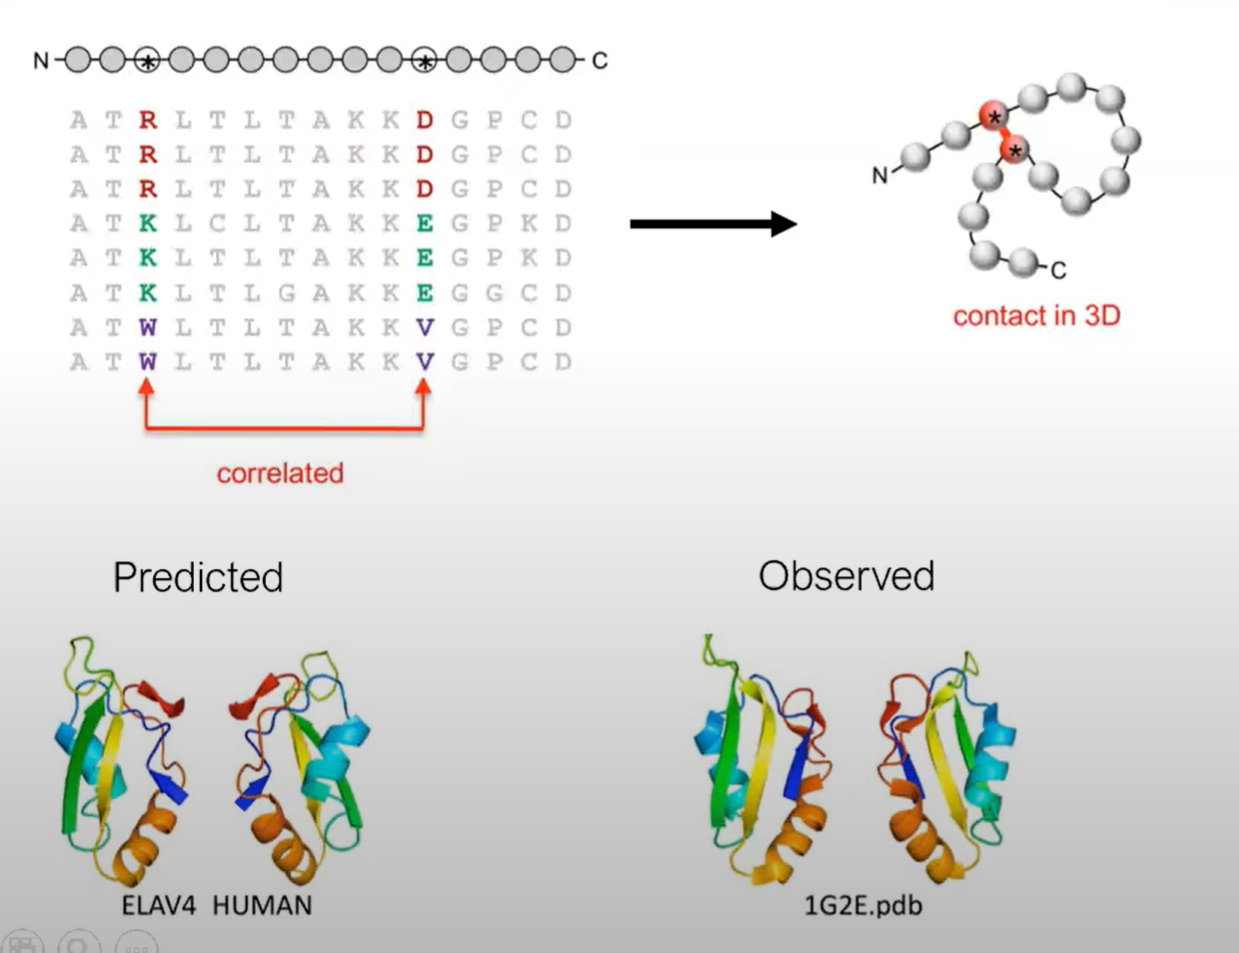
\includegraphics[width=\textwidth]{images/stdetr.png}};
                \node[](alpic) at (0,3.5) {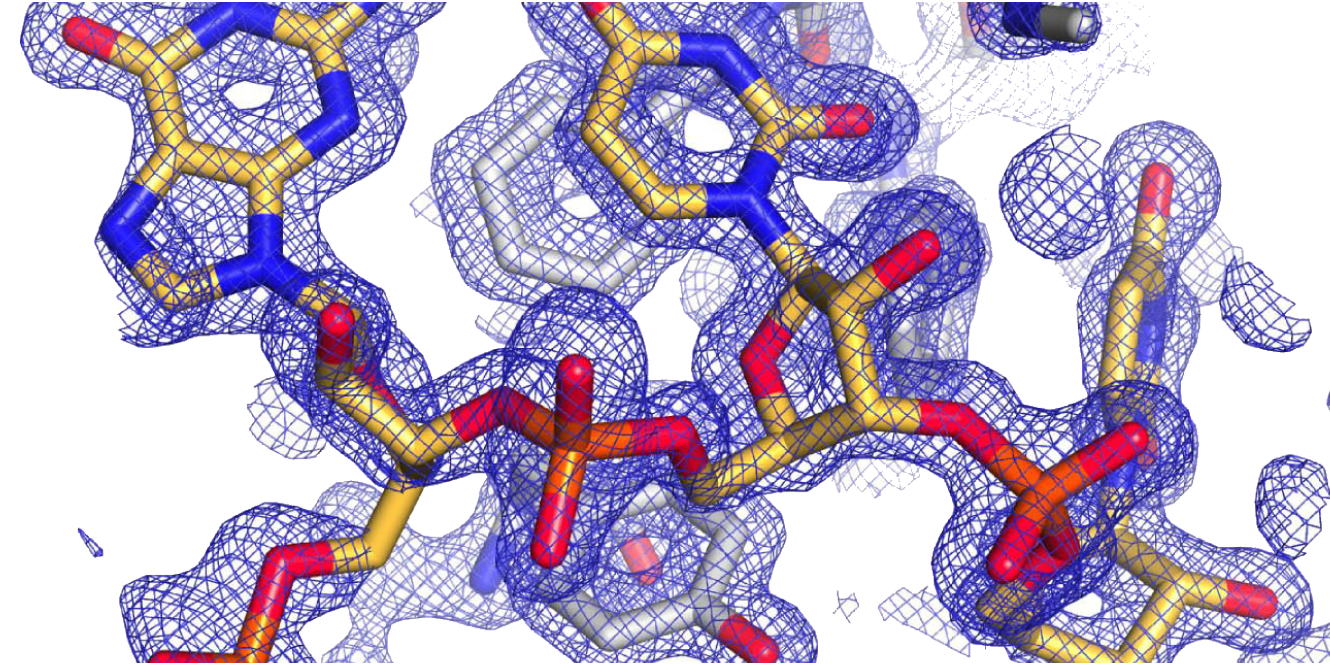
\includegraphics[width=5cm, keepaspectratio]{images/structural_data.PNG}};
            }
             \only<2>{
                \node[](pipic) at (0,3.5) {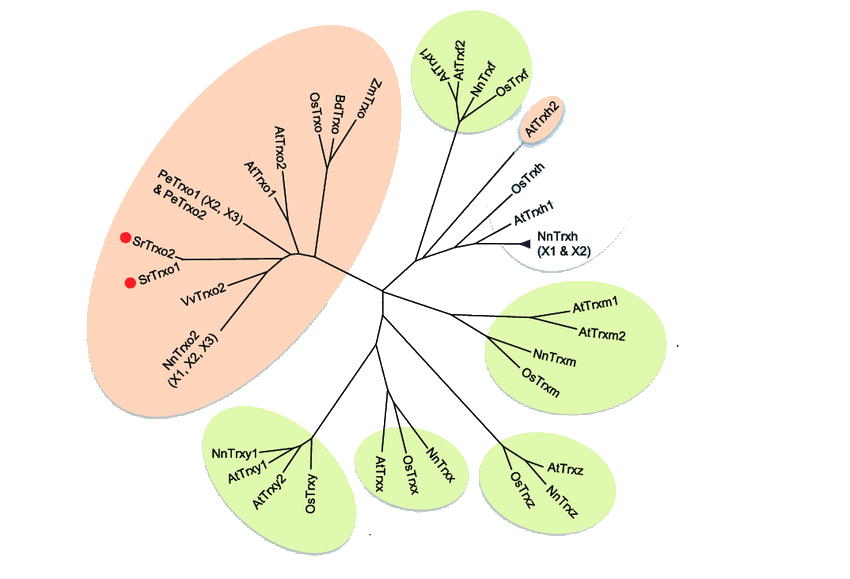
\includegraphics[width=5cm, keepaspectratio]{images/zero_shot_learning.PNG}};
            }
            \only<3>{
               \node[] (mutpic) at (0,3.5) {
\includegraphics[width=5cm, keepaspectratio]{images/efficiency.PNG}};
            }

            \only<4>{
                \node[] (mutpic) at (0,3.5) {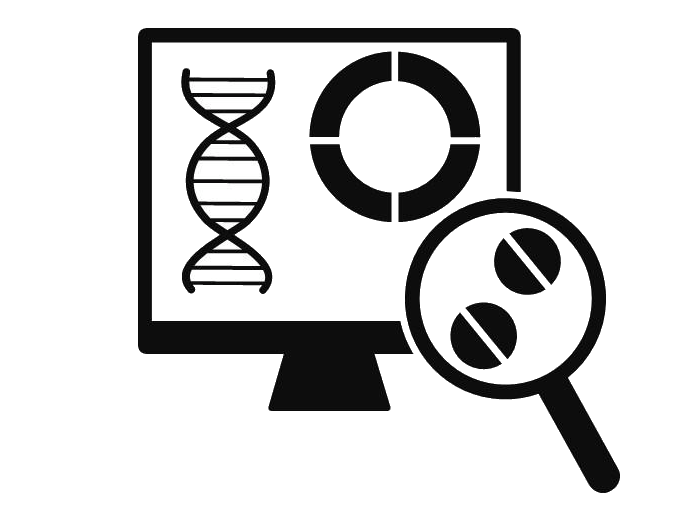
\includegraphics[width=5cm, keepaspectratio]{images/drug_discovery.PNG}};
            }
            

        \end{tikzpicture}
        \end{center}
    \end{columns}
\end{frame}



